
\section{Innovation and Usefulness}
The innovative idea behind this project is to make a physical notice board virtual, that can be
viewed anytime and anywhere immediately at the time when it is posted. This application also
helps to maintain the record of previous notices. You can make various groups like College
Notices, Event Notices of Societies, Library Notices, Placement Regarding Notices and many
other. The user subscribed to any group will get notify when any new notice is posted on it. User
can also respond to the notice if require.\\ 
This application has many uses. It cannot be used in college only but can also be used in Office
Places. It can also act as a market place by advertising about the various products and
technologies.

\begin{figure}[H]
\centering 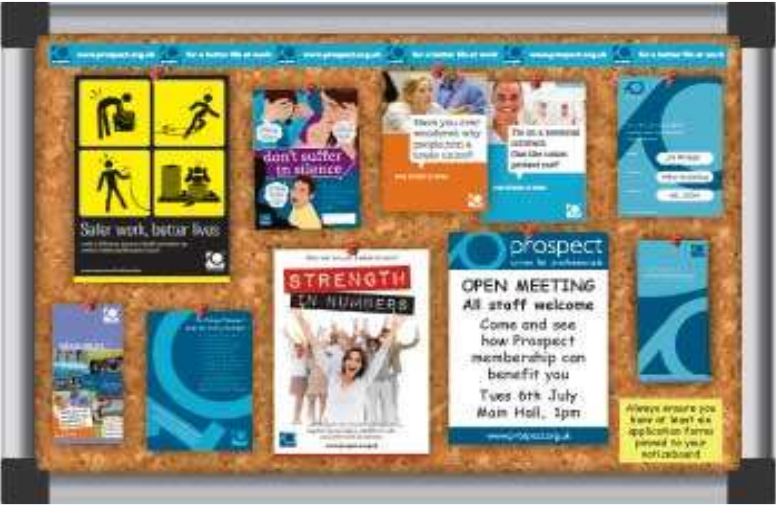
\includegraphics[scale=0.5]{image/notice.png}
\caption{DashBoard of Notices}
\end{figure}
\subsection{Features of Application}
\begin{enumerate}
\item \textbf{\emph{Sign In Using Google or Facebook Accounts:}}\\
 There is no need of registering for this
application. User can use his or her Google or Facebook account to login into this application. So
it relaxes you from learning new id and password.
\item \textbf{\emph{Sticky Notes:}}\\
User also have sticky notes facility through which a user can make a note of any
useful notice while reading the noticeboard. It will help him/her in remembering any of the
useful information regarding events going on in the college.
\item \textbf{\emph{Drag and Drop Notes:}}\\
It also allows you to drag and drop any PDF file, image or a video to
a vitual board that can be viewed by all. It helps and save you from writing lengthy notices again
and again.
\item \textbf{\emph{Customized Boards:}}\\
In this application, user can change the color of notice board or can
apply a decent background of his/her own choice.
User Preferences: User can also set who all can view the notice and who all can edit or post
the notices. The entire work will be under the control of admins of various groups and
departments.
\end{enumerate}
